\section{Preliminaries}
\label{sec:Preliminaries}
Let $\F$ be the set of floating-point numbers. Given
\begin{itemize}
\item a cluster of $p$ \glspl{pe} indexed with a rank $i \in \{0, \ldots, p - 1\}$ and interconnected by a \gls{mpi}
\item $n_i$ floating-point numbers (elements) on the \gls{pe} with index $i$ ($N := \sum_{i=0}^{p-1} n_i$ in total)
\item a not necessarily associative binary operation $\circ: \F \times \F \rightarrow \F$
\end{itemize}
we want to reduce all numbers by means of $\circ$ so that the end result is bitwise-reproducible.
A reduction algorithm is called bitwise-reproducible if multiple executions over the same set of numbers with a variable number of \glspl{pe} produce bit-per-bit the exact same results.

In order to correctly distribute the $N$ elements over $p$ \glspl{pe}, we need to deal with cases where $N$ is not divisible by $p$.
Let $a := \lfloor \tfrac{N}{p} \rfloor$ be the rounded number of elements per \gls{pe}.
We can assign the remaining $N \bmod p$ elements to the upper or lower ranks:
\begin{align}
\label{eq:lowerDistribution}
n_i^{\textrm{lower}} &= \begin{cases}
    a + 1 & \textrm{if } i < N \bmod p \\
    a & \textrm{otherwise}
\end{cases} \\
\label{eq:upperDistribution}
n_i^{\textrm{upper}} &= \begin{cases}
    a & \textrm{if } i < N - (N \bmod p) \\
    a + 1 & \textrm{otherwise}
\end{cases}
\end{align}

\section{Related Work}
\label{sec:RelatedWork}

\subsection{Sequential left-to-right reduction}
\label{sec:SequentialLeftToRightReduction}


A naive approach to solving above problem is to gather all elements on a single PE and then apply the reduction operation strictly from left to right:

\begin{equation}
x_0 \circ x_1 \circ x_2 \circ \ldots  \circ x_{N-1} = ((x_0 \circ x_1) \circ x_2) \circ \ldots
\end{equation}

While simple in implementation, this approach suffers from one major drawback:
It does not benefit from any parallelization whatsoever.
Because of the communication overhead, performance decreases with an increasing number of \glspl{pe}.


\subsection{Reproducible Accumulators}
\label{sec:Reproducible Accumulators}
For floating-point summation in particular, Ahrens et al.\ have developed an algorithm that uses a 6-word reproducible accumulator to avoid unpredictable rounding errors.\cite{ahrens_algorithms_2020}
After reading all the input data, the summation can occur in parallel in no particular order and still produces bitwise identical results.
This requires around $9N$ floating-point operations and $3N$ bitwise operations.
The Reproducible Basic Linear Algebra Subprograms (ReproBLAS) software package implements this algorithm and exposes a user-friendly API.\@

Naturally, this approach is not suitable for general reduction operations, since it depends on specific properties of floating-point numbers as specified in the IEEE 754 standard \cite{noauthor_ieee_nodate-1}.


\subsection{Reduction Tree}
\label{sec:ReductionTree}

\begin{figure}[H]
\centering
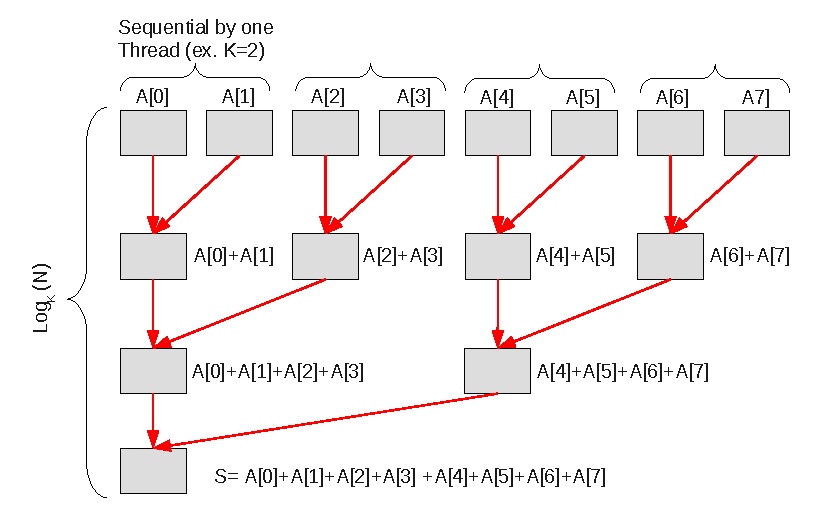
\includegraphics[scale=0.7]{figures/villa_et_al_reduction_tree.pdf}
\caption{General reduction tree (figure from Villa et al. \cite{villa_effects_2009})}
\label{fig:villa_reduction_tree}
\end{figure}


Villa et al.\ have utilized a $K$-ary tree structure on a Cray XMT system to sum floating-point numbers reproducibly \cite{villa_effects_2009}.
Figure \ref{fig:villa_reduction_tree} gives a schematic overview of the calculation order.
Using parallel-prefix accumulation, they compute the sum of $N$ summands in $\log_K (N)$ steps, where $K$ determines how many numbers are accumulated sequentially in each step.
The reproducibility stems from the fact that the reduction tree only depends on the total number of summands $N$ and the constant $K$, therefore the same calculation order is used even if the cluster size differs.

The original source code is not available even after contacting the authors, therefore the exact inner workings of this algorithm and runtime comparisons are subject to speculation only.
